\section{Database Model / Classes} \label{DataBaseModel/Classes}
\Cref{DatabaseModel} shows a diagram of the relationship between classes in the database model.

\begin{figure}[H]
	\centering
    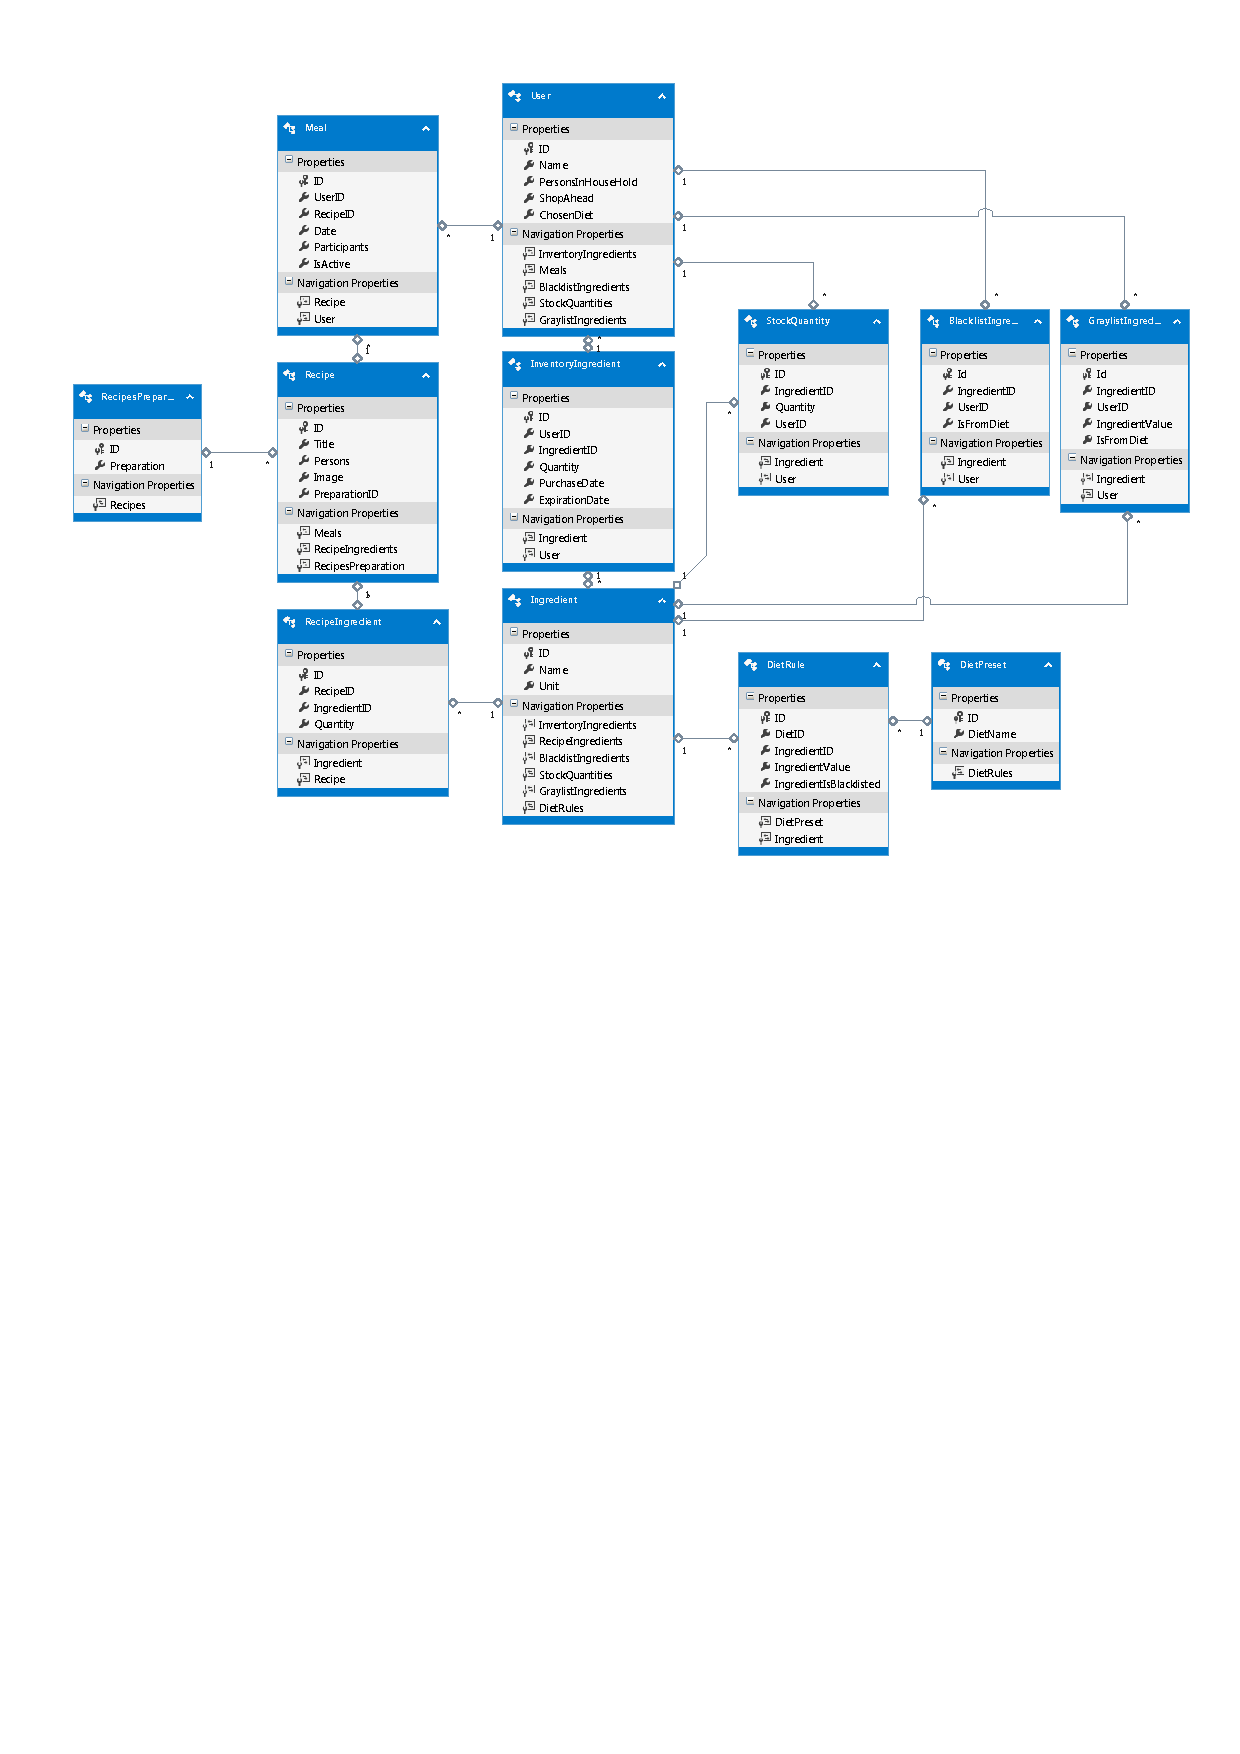
\includegraphics[width=1\textwidth, trim=0 350 0 0]{Grafik/FoodDatabase.pdf}
	\caption{Relationship between classes in the database model.}
	\label{DatabaseModel}
\end{figure}

\textbf{Recipe} is a class that describes the individual recipes. The Persons property describes how many person this recipe was originally intended for. It has a onerelates to the class RecipePreperation, by having one property, and to RecipeIngredient, by having a list of RecipeIngredient. 

The \textbf{Ingredient} class describes a food and which unit is used to measure it such as kg or ml.

\textbf{RecipePreparition} is a class used exclusively to hold a string property \textit{Preparation} which is a text guide on how to prepare the recipe. The reason this is not just a string property in the Recipe class, is to allow lazy-loading this property from the database when it is needed, thereby allowing the program to list different recipes without having to download a lot of text data that is not displayed.

\textbf{RecipeIngredient} is a class that wraps the Ingredient class to add the quantity property that keep track of how much a recipe needs of the specific ingredient. In the database it also serves a a junction table that connects a Recipe with and Ingredient.

The \textbf{InventoryIngredient} class describes food that a user can buy or have in the inventory. It is very similar to the \textbf{RecipeIngredient} class, but has a \textit{ExpirationDate} property as well, since it is used to describe real existing food, unlike the \textbf{RecipeIngredient} class which describes food is needed.

The \textbf{Meal} class describes a scheduled meal in a user's mealplan. It contains information about the recipe that defines the meal, how many participants who will be eating, and when it is scheduled for. The \textit{IsActive} property tells if this meal has already been eaten and thereby archived. This usually means that the meal is scheduled for a date within the past.

The \textbf{User} class is primarily used to keep preferences about a user, such as a list of \textbf{Meals} which is what the mealplan consists of. The preferences include \textit{PersonsInTheHousehold}, \textit{ChosenDiet} and \textit{ShopAhead} which is how many days the shopping list should take into consideration when generating the list. The User is identified with a \textit{Name} as well, but other personal details is not taken into consideration at this time in this project.

\textbf{StockQuantity} is similar to the InventoryIngredient class because it contains information about an ingredient and a quantity. It is used as a user preference to keep track of ingredients that a user always want a certain amount of. If the inventory go below this setting the ingredient will automatically be added to the shopping list.

\textbf{BlacklistIngredient} and \textbf{GraylistIngredient} is like \textbf{StockQuantity} used for user preferences. The \textbf{BlacklistIngredient} class contain information about ingredients that the user does not want to appear in a recipe, and \textbf{GreylistIngredient} is used to rate and ingredient to adjust it's impact in the search.

The \textbf{DietPreset} class is used for link the \textbf{DietRules} to the specific diet. This is done by useing the id from the DietPreset and an id from an ingredient and saveing them in the \textbf{DietRule} class. Specifying if the ingredient is either blacklisted or graylisted is needed. Only if the item is graylisted is the ingredient value should be set. 




